\documentclass[a4paper]{article}

\usepackage[english]{babel}
\usepackage[utf8x]{inputenc}
\usepackage{amsmath}
\usepackage{amsfonts}
\usepackage{graphicx}
\usepackage[]{algorithm2e}
\usepackage[colorinlistoftodos]{todonotes}
\usepackage[hidelinks]{hyperref}

\newcommand{\itab}[1]{\hspace{0em}\rlap{#1}}
\newcommand{\tab}[1]{\hspace{.2\textwidth}\rlap{#1}}

\title{CS 5785 -- Applied Machine Learning -- Lec.\ 19}
\author{Prof.\ Nathan Kallus, Cornell Tech\\Scribe: TBD}
\date{November 7, 2017}

\begin{document}
\maketitle

\section{Neural Networks}
Neural networks were developed separately from the statistics community, but they are nearly identical models to something from statistics called Projection Pursuit Regression (PPR). PPR was introduced in 1981, but didn't flourish, probably due to computational demands, but it has blossomed in its reincarnation in the field of neural networks. Neural networks are sometimes called ``artificial neural networks" since actual neurons have numerous subtle properties that are not captured by the commonly used simple model.

\subsection{``Vanilla" Neural Networks}
We start with what HTF call the ``vanilla" neural network. This is also referred to as the \emph{single hidden layer back-propagation network} or \emph{single layer perceptron}.
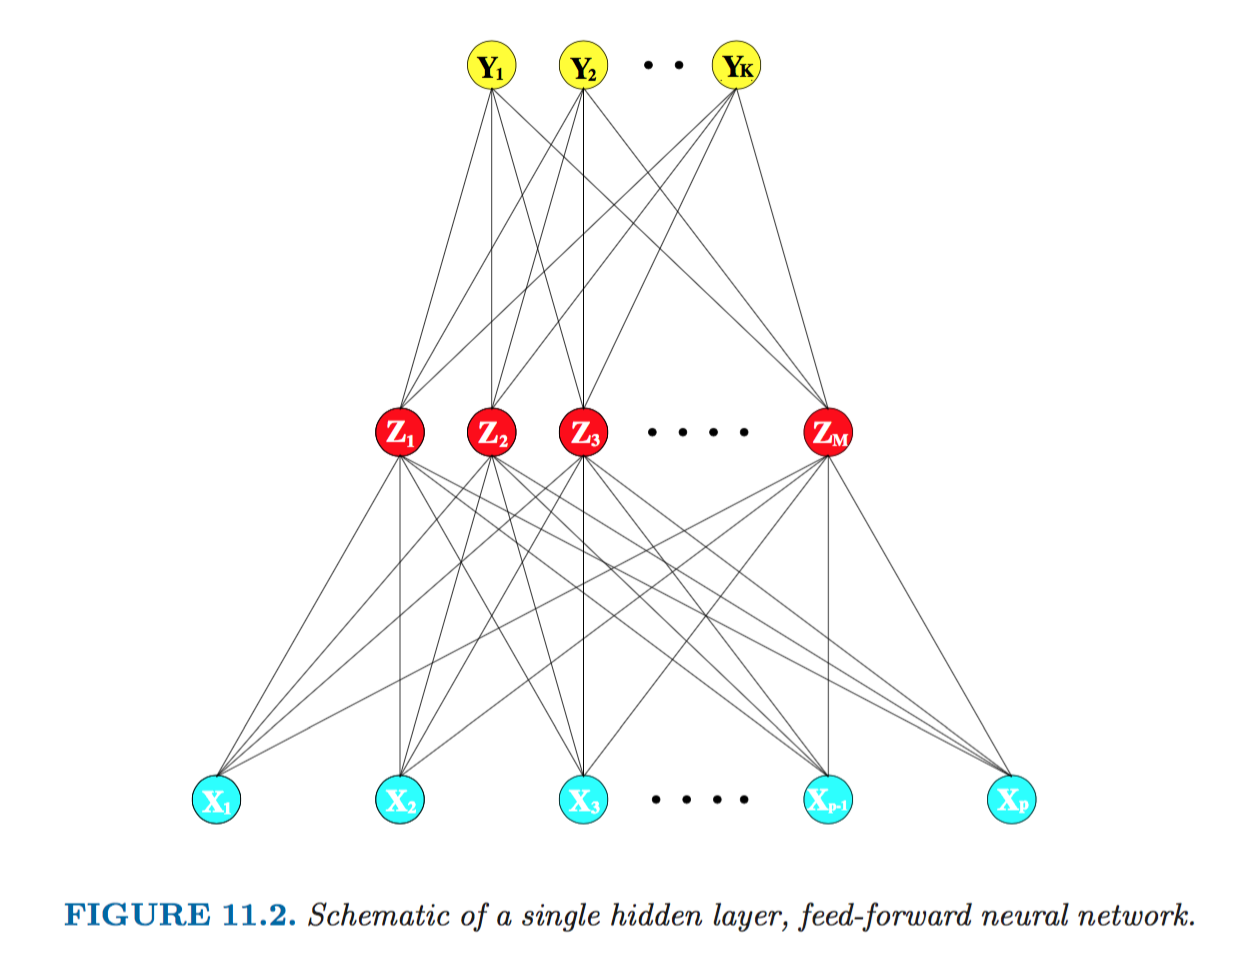
\includegraphics[width=\textwidth]{VanillaNN.png}
\\\\
Neural networks can be used for both classification and regression. For classification, we use ${K}$ units at the top, one for each class. For the case of MNIST digits, we have ${K=10}$. This gives us ${K}$ target measurements ${y_k}$, ${k=1,...,K}$, each coded as 0 or 1 for the ${k}$th class. This is also known as a \emph{one-hot encoding}. The $K$ units in the output layer model the probabilities of each class. \\\\
The computation effected by this network is as follows:
\begin{itemize}
  \item $Z_m=\sigma(\alpha_{om}+\alpha_m^\top X),\ m=1,...,M$
  \item $T_k=\beta_{0k} + {\beta_k^\top Z},\ k=1,...,K$
  \item $f_k(X) = g_k(T),\ k=1,...,K$
  \item where $Z = (Z_1, ...,Z_M)$ and $T = (T_1,...,T_K)$
\end{itemize}
The activation function $\sigma(v)$ is usually chose to be sigmoid, $\sigma(v) = \frac{1}{1+e^{-v}}$, which we've seen before. It is nicely differentiable -- a property we will soon exploit.
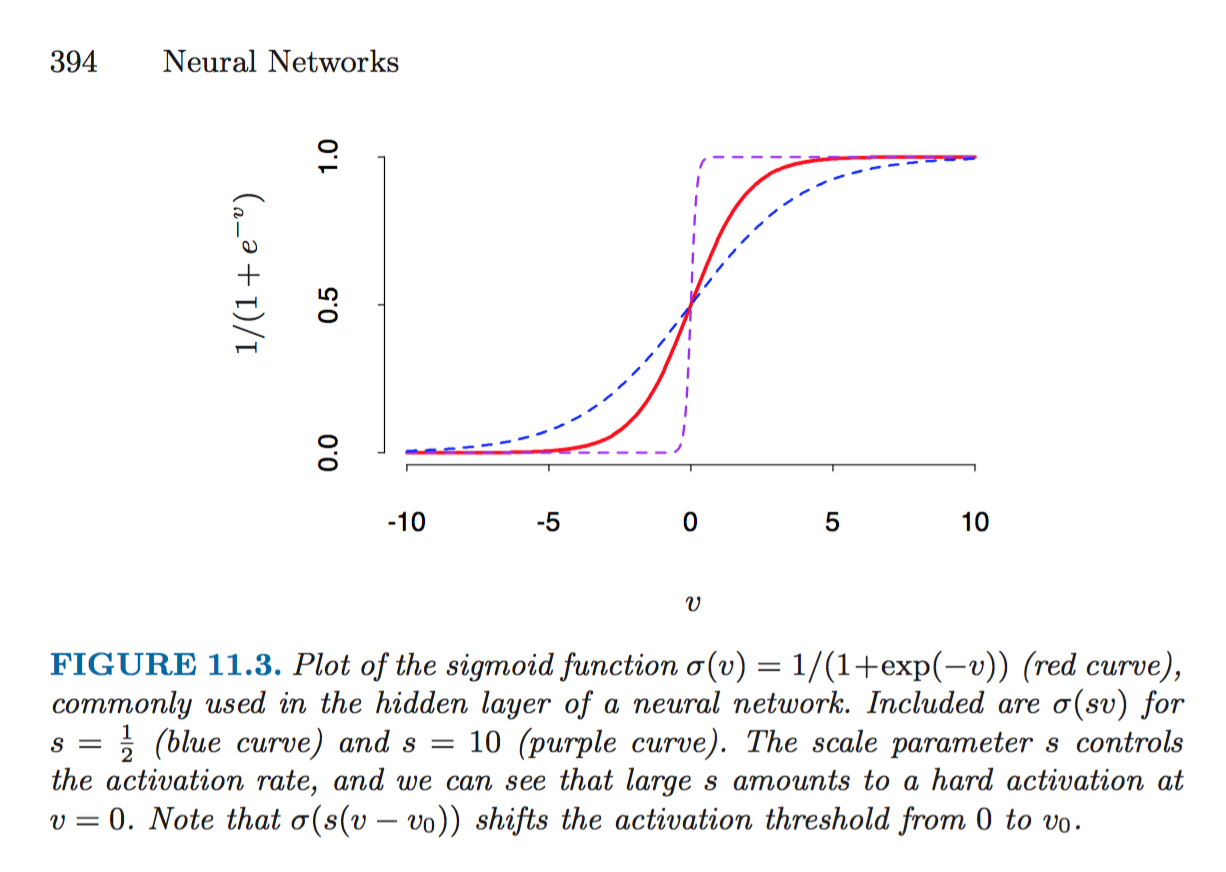
\includegraphics[width=\textwidth]{SigmoidNN.png}
As we saw before with linear regression, we can absorb the offset terms $\alpha_{0k}$ and $\beta_{0k}$ by considering the constant 1 as an additional input feature. This makes notation cleaner.

The output of the function $g_k(T)$ allows a final transformation of the vector of outputs $T$; typically this is a softmax function:

\begin{align*}
g_k(T) = \frac{e^{T_k}}{\sum_{l=1}^K e^{T_l}}
\end{align*}

Softmax ensures that the density output is non-negative and sums to 1. It is the same transformation used in the multilogit model (Sec.\ 4.4). We only studied the 2-class case at the time, when we covered logistic regression.
\\ \\
Logistic regression is similar to using just one of the hidden layers.  The idea is that you could have some raw inputs coming in, but the inputs might benefit from a "basis transformation" after which simple linear regression could get us to the result we want.
\\ \\
The units in the middle, $Z_m, m=1,...,M$ are called hidden units since we don't observe them directly. In general, one can have more than a single hidden layer. We can think of the $Z_m$ as a ``basis expansion'' of the raw inputs $X$ -- the neural net is then a linear multilogit model using these transformations as inputs.

\subsection{Fitting a Neural Network}
Fitting a neural network means solving for the weights $\Theta$ consisting of:
\begin{align*}
\left \{ \alpha_{0m}, \alpha_m; m=1,2,...,M \right \} \qquad M(p+1)\quad  \text{weights}
\\ \\
\left \{\beta_{0k}, \beta_k; k=1,2,...,K \right \} \qquad K(M+1) \quad \text{weights}
\end{align*}

The appropriate measure of fit (i.e., error function) depends on the task.  Regression uses:
\begin{align*}
R(\Theta) = \sum_{k=1}^K\sum_{i=1}^N(y_{ik}-f_k(x_i))^2
\end{align*}
Note that this is sum of squares, with $f_k$ representing the neural net. For classification we usually use cross-entropy:
\begin{align*}
R(\Theta) = -\sum_{i=1}^N\sum_{k=1}^Ky_{ik}\log f_k(x_i)
\end{align*}
with classifier
\begin{align*}
G(X) = \arg\max_k\ f_k(x)
\end{align*}

In the case of softmax activation function and the cross-entropy error function, this is exactly a linear logistic regression model in the hidden units, and all the parameters are estimated by maximum likelihood.

\section{Back-Propagation}
Finding the global minimum of $R(\Theta)$ will probably result in overfitting to the training data. In practice we will need some form of regularization, either via penalty term or indirectly via early stopping. Applying gradient descent to $R(\Theta)$ has a special name: \textbf{back-propagation}. In purely mathematical terms, back-propagation is ``simply the chain rule" of differentiation. It is implemented as a forward and backward sweep over the network, keeping track only of quantities local to each unit.
\subsection{The Chain Rule}
Recall the chain rule: $\frac{dz}{dx} = \frac{dz}{dy}\frac{dy}{dx}$ when $z$ is a function of $y$ which is itself a function of $x$. This is not to be confused with chain rule of probability, which is useful in the study of Bayesian networks: $P(A,B,C) = P(A | B,C) P(B| C) P(C)$.

Let's examine back-propagation for the case of \emph{squared error} loss. Let ${z_{mi}=\sigma(\alpha_{0m}+\alpha^\top_{m}x_i)}$ and let $z_i=(z_{1i},z_{2i},...,z_{Mi})$. Recall that $i$ ranges over observations ($i=1,...,N$) and $k$ ranges over output units ($k=1,...,K$). Then we can write the cost function as
\begin{align*}
R(\theta)&=\sum_{i=1}^{N} R_i\\
&=\sum_{i=1}^N \sum_{k=1}^K (y_{ik}-f_k(x_i))^2
\end{align*}
Now we look at the derivatives with respect to the $\beta$s and $\alpha$s. Remember that the $\alpha$s act on the input features and the $\beta$s act on the hidden nodes.
\begin{align}
\frac{\partial R_i}{\partial \beta_{km}} &= -2(y_{ik}-f_k(x_i))g'_k(\beta^\top_kz_i)z_{mi}\\
\frac{\partial R_i}{\partial \alpha_{ml}} &= -\sum_{k=1}^K \underline{2(y_{ik}-f_k(x_i))g'_k(\beta^\top_kz_i)}\beta_{km}\sigma'(\alpha^\top_mx_i)x_{il}
 \end{align}
Next we apply a gradient descent update, expressed as:
\begin{align*}
\beta_{km}^{(r+1)} &= \beta_{km}^{(r)}-\gamma_r\sum_{i=1}^N \frac{\partial R_i}{\partial \beta_{km}^{(r)}}\\
\alpha_{ml}^{(r+1)} &= \alpha_{ml}^{(r)}-\gamma_r\sum_{i=1}^N \frac{\partial R_i}{\partial \alpha_{ml}^{(r)}}
\end{align*}
where $r$ is the iteration and $\gamma_r$ is the \emph{learning rate}. This can be a constant or something more interesting as a function of $r$ which we will discuss later.\\\\
To get more insight into what is happening in the gradient descent steps, let's use the following notation.
\begin{align*}
\frac{\partial R_i}{\partial \beta_{km}} &= \delta_{ki}z_{mi}\\
\frac{\partial R_i}{\partial \alpha_{ml}} &= s_{mi}x_{il}
\end{align*}
We can think of $\delta_{ki}$ and $s_{mi}$ as ``errors" arising from the current model at the output and hidden layer units respectively. Here is where the \emph{back-propagation} idea emerges. These errors satisfy:
\begin{align}
s_{mi}=\sigma'(\alpha_m^\top x_i)\sum_{k=1}^K \beta_{km}\delta_{ki}
\end{align}
How do we get this? Recall that the big portion of (2) comes from (1) (see above equations).
\begin{itemize}
  \item We call the underlined quantity multiplying $x_{il}$ in (2)  $s_{mi}$ and that, in turn, is a sum over the quantity multiplying $z_{mi}$ in (1) over all $K$.
  \item The term $\sigma'(\alpha_m^\top x_i)$ doesn't depend on $k$, so we can pull it out front.
\end{itemize}
$\Rightarrow$ This says how these two errors are related to one another.\\
Using this formalism, we can do the gradient descent updates using a 2-pass algorithm:
\begin{enumerate}
  \item Forward pass: fix the weights (the $\alpha$s and $\beta$s) and compute the predicted values which we denote $\hat{f}_k (x_i)$, i.e., the output of the neural net.
  \item Backward pass: compute the errors $\delta_{ki}$ and back propagate them using (3) to obtain $s_{mi}$.
  \item With $\delta_{ki}$ and $s_{mi}$ in hand, we can compute the gradients for the updates.
\end{enumerate}
Further explanation available in this video: \url{https://www.youtube.com/watch?v=Ilg3gGewQ5U}
\subsection{Discussion on Back-Propagation}
The nice feature of back-propagation is its simple, local nature.  Each hidden unit passes and receives information only to and from units that share a connection. This makes it particularly well suited for parallel computation.\\ \\
The gradient descent update we derived is a form of batch learning, with parameter updates being a sum over all training cases.  As we saw in the discussion on IRLS, we can drop the sum and update the gradient after each training case (Stochastic Gradient Descent).
\begin{itemize}
  \item Whereas $\gamma_r$ is usually chosen (after some simple optimization) to be a constant in the batch case, in the stochastic case $\gamma_r \rightarrow 0$ as $r \rightarrow 0$.
  \item Second order techniques (like Newton-Raphson) are problematic since the Hessian of $k$ is too big.
\end{itemize}
There are many, many tricks of the trade that exist for speeding up back-propagation, however we will not be covering them in this class. \\ \\
We need to understand that these models are generally overparameterized (parameters $>$ input) and sometimes dramatically so. This makes them susceptible to overfitting, and the optimization problem is nonconvex.  Other issues include: input scaling, weight decay (and other forms of regularization), number of hidden layers, and hidden units.  As HTF says, ``There is quite an art in training neural networks". $\ddot\smile$


\end{document}
